\documentclass[11pt]{article}
\usepackage[letterpaper,margin=0.8in]{geometry}
\usepackage{enumitem,array,booktabs,xcolor,tikz,amssymb,amsmath}
\usetikzlibrary{calc,patterns,decorations.pathmorphing,arrows.meta}
\usepackage{needspace}
\usepackage[T1]{fontenc}\usepackage{lmodern}
\setlength{\parindent}{0pt}\setlength{\parskip}{5pt}
\renewcommand{\arraystretch}{1.5}
\newif\ifkey \input{mode}
\newcommand{\ans}[2][1]{\ifkey{\color{red!70!black}\itshape #2}\par\else\par\foreach\i in{1,...,#1}{\vspace{0.75cm}\noindent\rule{\linewidth}{0.4pt}\par}\fi}
\newcommand{\work}[2][3cm]{\ifkey{\color{red!70!black}\itshape #2}\par\else\par\vspace{#1}\fi}
\newcommand{\fa}[1]{\ifkey{\color{red!70!black}\bfseries #1}\else\fi}
\newcommand{\blank}[2][2.5cm]{\ifkey\fa{#2}\else\rule{#1}{0.4pt}\fi}
\newcommand{\pts}[1]{\hfill{\small[#1]}}
\newcommand{\sect}[1]{\par\needspace{12\baselineskip}\vspace{8pt}\noindent{\large\bfseries #1}\par\vspace{-4pt}\noindent\rule{\linewidth}{0.8pt}\par}
\newcommand{\q}[1]{\par\needspace{8\baselineskip}\vspace{6pt}\noindent\textbf{#1}\ }
\newcommand{\sub}[1]{\par\vspace{3pt}\hspace*{1em}(#1)\ }
\tikzset{grnd/.style={pattern=north east lines,draw=none},
  frc/.style={-{Stealth[length=7pt]},very thick,red!70!black}}

\pagestyle{plain}
\begin{document}
\begin{document}
\ifkey{\color{red!70!black}\bfseries ANSWER KEY}\par\fi
{\LARGE\bfseries Forces Quiz: Friction, Inclines, Systems and Springs}\par\vspace{6pt}
Name: \rule{6.5cm}{0.4pt}\hfill Date: \rule{3cm}{0.4pt}\par
Calculators allowed. Show your work and units. Use $g = 9.8\ \text{m/s}^2$. Total: 28 points.

\begin{center}\fbox{\parbox{0.9\linewidth}{\centering
$\Sigma F = ma \qquad W = mg \qquad f_k = \mu_k N \qquad f_s \le \mu_s N \qquad F = kx$}}\end{center}

\sect{Friction}
\q{1.} An 18 kg crate sits on a floor. $\mu_s = 0.35$ and $\mu_k = 0.20$.
\sub{a} What is the largest static friction the floor can give? \pts{1} \hfill \blank{61.7 N ($0.35 \times 176.4$)}
\sub{b} You push with 45 N and the crate does not move. How big is the friction force? \pts{2}
\ans{45 N. The crate stays at rest, so static friction matches the push; 61.7 N is only its limit.}
\sub{c} You push with 80 N instead. Does it move? If so, find its acceleration. \pts{3}
\work[3cm]{80 N beats 61.7 N, so it slides (1). $f_k = 0.20 \times 176.4 = 35.3$ N (1). $a = (80 - 35.3)/18 = 2.5\ \text{m/s}^2$ (1).}

\q{2.} Why does it take a bigger push to start the crate sliding than to keep it sliding? \pts{1}
\ans{The largest static friction ($\mu_s N$) is bigger than kinetic friction ($\mu_k N$), because $\mu_s > \mu_k$.}

\sect{Inclines}
\q{3.} An 8.0 kg block sits on a frictionless ramp tilted at $35^\circ$.\par
\begin{center}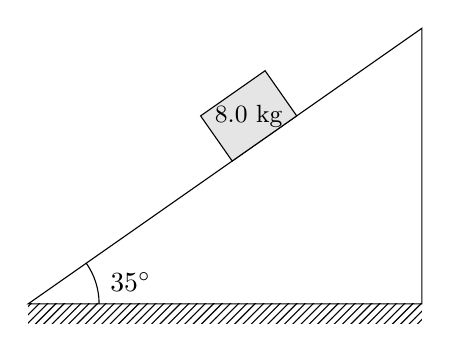
\begin{tikzpicture}
\fill[grnd] (0,-0.25) rectangle (5,0);
\draw (0,0)--(5,0)--(5,3.5)--cycle;
\draw (0.9,0) arc (0:35:0.9); \node at (1.3,0.28) {$35^\circ$};
\begin{scope}[shift={(3,2.1)},rotate=35]\draw[fill=gray!20] (-0.5,0) rectangle (0.5,0.7) node[midway]{\small 8.0 kg};\end{scope}
\end{tikzpicture}\end{center}
\sub{a} Draw the free-body diagram of the block on the picture. \pts{2}
\ans{Weight straight down; normal force perpendicular to the ramp. No friction.}
\sub{b} Find the part of the weight along the ramp. \pts{1} \hfill \blank{45 N ($78.4\sin 35^\circ$)}
\sub{c} Find the normal force. \pts{1} \hfill \blank{64 N ($78.4\cos 35^\circ$)}
\sub{d} Find the block's acceleration. \pts{1} \hfill \blank{$5.6\ \text{m/s}^2$ down the ramp}

\q{4.} A 2.0 kg block and a 6.0 kg block slide down the same frictionless ramp. Which has the bigger acceleration? Why? \pts{1}
\ans{Neither: $a = g\sin\theta$. The heavier block is pulled harder but needs just as much more force to speed up.}

\sect{Connected objects}
\q{5.} A 4.0 kg cart on a frictionless table is tied to a 1.2 kg mass hanging over an ideal pulley.\par
\begin{center}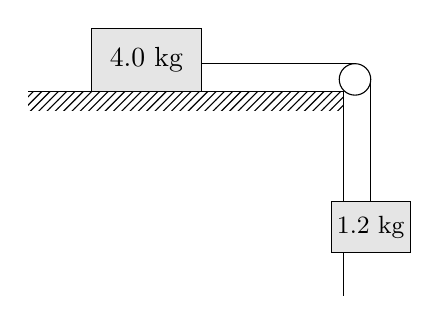
\begin{tikzpicture}
\fill[grnd] (0,-0.25) rectangle (4,0); \draw (0,0)--(4,0)--(4,-2.6);
\draw[fill=gray!20] (0.8,0) rectangle (2.2,0.8) node[midway]{4.0 kg};
\draw (4.15,0.15) circle (0.2); \draw (2.2,0.35)--(4.15,0.35); \draw (4.35,0.15)--(4.35,-1.4);
\draw[fill=gray!20] (3.85,-1.4) rectangle (4.85,-2.05) node[midway]{\small 1.2 kg};
\end{tikzpicture}\end{center}
\sub{a} Before calculating: will the tension be more than, less than, or equal to the hanging mass's weight once it moves? Why? \pts{1}
\ans{Less: the hanging mass speeds up downward, so its weight must beat the tension.}
\sub{b} Find the acceleration. \pts{2}
\work[2.2cm]{$a = \dfrac{1.2 \times 9.8}{5.2} = 2.26\ \text{m/s}^2$.}
\sub{c} Find the tension. \pts{2}
\work[2.2cm]{$T = 4.0 \times 2.26 = 9.0$ N. Check: $1.2(9.8 - 2.26) = 9.0$ N.}

\q{6.} An Atwood machine: a 7.0 kg mass and a 3.0 kg mass hang on either side of an ideal pulley. Find the acceleration and the tension. \pts{4}
\work[3.4cm]{$a = \dfrac{(7.0 - 3.0)(9.8)}{10.0} = 3.92\ \text{m/s}^2$ (2). For the 3.0 kg mass: $T - 29.4 = 3.0 \times 3.92$, so $T = 41.2$ N (2). Check: $68.6 - T = 7.0 \times 3.92$, $T = 41.2$ N.}

\sect{Springs}
\q{7.} A student hangs weights on a spring and measures the stretch.\par
\begin{center}\begin{tabular}{|l|*{4}{>{\centering\arraybackslash}p{1.4cm}|}}\hline
Force (N) & 0 & 1.5 & 3.0 & 4.5\\\hline
Stretch (m) & 0 & 0.020 & 0.040 & 0.060\\\hline
\end{tabular}\end{center}
\sub{a} Find the spring constant $k$. \pts{2} \hfill \blank{75 N/m ($1.5/0.020$)}
\sub{b} Predict the stretch when a 0.80 kg mass hangs at rest on this spring. \pts{2}
\work[2.2cm]{$F = mg = 7.84$ N; $x = 7.84/75 = 0.10$ m.}

\q{8.} A spring scale with $k = 150$ N/m sits in the string of question 5.
\sub{a} While the cart is held still, what does the scale read? \pts{1} \hfill \blank{11.8 N ($mg$ of the hanging mass)}
\sub{b} Once the cart is let go, how far does the scale stretch? \pts{1} \hfill \blank{0.060 m ($9.0/150$)}
\end{document}
